\documentclass[11pt, twoside]{article}
\input{commandsFile}
\raggedbottom 
\begin{document}

%====================================================
% TITLE PAGE
%====================================================
\begin{titlepage}
\begin{center}

% Logo
\vspace*{1cm}
\includegraphics[scale=0.5]{Images/PolimiLogo}

\vspace{1cm}

% University name
{\Large \textbf{POLITECNICO DI MILANO}}\\
\vspace{0.2cm}
{\large 1863}

\vspace{1.2cm}

% Degree and course
{\Large \textbf{Computer Science and Engineering}}\\
\vspace{0.3cm}
{\Large \textbf{Software Engineering II}}\\
\vspace{0.3cm}
{\large 2025 -- 2026}

\vspace{1.5cm}

% Document type
{\Huge \textbf{DD}}\\
\vspace{0.4cm}
{\Large \textbf{Design Document}}\\
\vspace{0.3cm}
{\large \textbf{\textit{Best Bike Paths(BBP)}}}
\vfill

% Project and authors
{\small
\textbf{By}\\
\vspace{0.2cm}
Jayasurya Marasani (11023924)\\
Arunkumar Murugesan (11051547)\\
Sneharajalakshmi Palanisamy (11132155)

}

\vspace{1cm}

\end{center}
\end{titlepage}


%Define deliverable specific info
%Replace cell contents where needed
\begin{table}[h!]
\begin{tabu} to \textwidth { X[0.3,r,p] X[0.7,l,p] }
\hline

\textbf{Deliverable:} & DD\\
\textbf{Title:} & Design Document \\
\textbf{Authors:} & Jayasurya Marasani, Arunkumar Murugesan and Sneharajalakshmi Palanisamy \\
\textbf{Version:} & 1.0 \\ 
\textbf{Date:} & 07 January 2026 \\
\textbf{Download page:} & https://github.com/BBPpolimi/MurugesanPalanisamyMarasani \\
\textbf{Copyright:} & Copyright © 2025, Jayasurya Marasani, Arunkumar Murugesan and Sneharajalakshmi Palanisamy – All rights reserved \\
\hline
\end{tabu}
\end{table}




\setcounter{page}{2}


%------------------------------------------------------------------------------------------------------------------------------------------------
\newpage
\addcontentsline{toc}{section}{Table of Contents}
\tableofcontents
\newpage
\addcontentsline{toc}{section}{List of Figures}
\listoffigures
\addcontentsline{toc}{section}{List of Tables}
\listoftables

%------------------------------------------------------------------------------------------------------------------------------------------------
\clearpage
{\color{Blue}{\section{Introduction}}}
\label{sect:introduction}
Cycling has seen accelerated adoption in recent years due to a combination of post-pandemic mobility shifts, increased climate awareness, urban congestion, expanded micro-mobility options and sustained public investment in cycling infrastructure. As a result, cycling is increasingly used for both commuting and daily travel, supported by measurable growth in usage and policy targets aimed at further expansion. However, despite this growth, most widely used navigation tools remain optimized for motor vehicles and do not adequately represent factors that determine cycling safety and comfort, such as surface quality, obstacles, changing conditions, or cyclist-specific risk areas. Consequently, existing maps can indicate where to ride, but not whether a route is suitable or safe for cyclists.

Best Bike Paths (BBP) addresses this gap by providing a cyclist-first navigation system focused on route quality, safety and real-world riding conditions. The application enables users to record and store trips with computed statistics, contribute and validate information about bike paths through manual input and automated trip recording with obstacle detection and search for routes ranked using consolidated quality indicators rather than distance alone. Path conditions are visualized using an explicit scoring model, allowing cyclists to quickly assess comfort and risk, while dynamic updates ensure that changing conditions are reflected over time. BBP also supports guest usage, enabling quick access to bike-friendly routing without mandatory registration.


\noindent Best Bike Paths (BBP) is a mobile application system that enables users to:
\begin{enumerate}
	\item Record bicycle trips and store them in a personal trip log with computed statistics.
	\item Contribute information about bike paths, including segment condition and obstacles, through manual reports and confirmed automatic detection.
 	\item Query and compare routes between two points, ranking candidate paths based on both route effectiveness (e.g., distance, elevation, turns) and path quality indicators derived from consolidated reports.
	\item Use the system as guest users to obtain a fast and easy route from point A to point B without requiring registration.
\end{enumerate}

\subsection{Scope}
BBP is a mobile first application that interacts with the user's device capabilities (GPS, accelerometer, gyroscope and network connectivity) and integrates external services (maps/routing and weather) to support both individual trip logging and community-maintained bike path information.

The system scope includes:

\begin{enumerate}
	\item \textbf{User management}
	\begin{itemize}
		\item User registration and login.
		\item Role-based access for administrative features.
	\end{itemize}
	\item \textbf{Trip recording and personal log}
	\begin{itemize}
		\item Real-time trip tracking using GPS.
		\item Automatic computation and storage of trip statistics (e.g., distance, duration, average speed).
		\item Trip saving and review through a personal trip history.
	\end{itemize}
	\item \textbf{Optional Trip Enrichment}
	\begin{itemize}
		\item Retrieval and attachment of weather information to trips when the weather service is reachable.
	\end{itemize}
	\item \textbf{Manual Bike Path Contributions}
	\begin{itemize}
		\item Manual input of bike path information, including streets/segments, segment condition/status, and obstacles.
		\item Ability to edit or remove user-submitted reports as allowed by permissions.
	\end{itemize}
	\item \textbf{Automatic Aquistion of Bike Path Data}
	\begin{itemize}
		\item Collection of GPS traces and sensor events (accelerometer/gyroscope) during trip recording when automatic mode is enabled.
		\item Detection of candidate issues (e.g., potholes/roughness indicators) based on sensor patterns.
	\end{itemize}
	\item \textbf{User Confirmation Workflow}
	\begin{itemize}
		\item Presentation of automatically detected candidate issues after a trip.
		\item User confirmation, rejection, or correction of detected issues before they are stored as publishable path reports.
	\end{itemize}
	\item \textbf{Path Search and visualization for all Users}
	\begin{itemize}
		\item Route search between origin and destination for guest and registered users.
		\item Ranking of candidate routes by a path score that combines route effectiveness (e.g., distance/elevation/turns) and path quality (segment status and obstacles).
		\item Map-based visualization of selected routes with overlays for segment condition and reported obstacles.
	\end{itemize}
	\item \textbf{Report merging and consolidated status}
	\begin{itemize}
		\item Periodic merging of multiple user's reports into consolidated segment status information, applying freshness and majority/weighted-majority logic.
	\end{itemize}
	\item \textbf{Administration and data quality controls}
	\begin{itemize}
		\item Administrative ability to block users who repeatedly submit false data.
		\item Administrative ability to remove or hide problematic reports/obstacles and keep the consolidated data consistent.
	\end{itemize}
\end{enumerate}


\subsection{Definitions, Acronyms, Abbreviations}
\subsubsection{Definitions}

\begin{enumerate}
  \item \textbf{Flutter}:  A cross-platform UI framework used to build native mobile apps from a single codebase (Android and iOS). In BBP it is used to implement UI elements and access to device sensors through plugins. 
  
  \item \textbf{Firebase/FlutterFire}: Firebase is Google's backend platform. FlutterFire is the official set of Flutter plugins to use Firebase services. In BBP it provides authentication, database, file storage, server-side logic and (optionally) push notifications.

  
  \item \textbf{MapService(RoutesAPI)}: An external mapping service providing geocoding (address → coordinates) and routing (candidate routes between two points). In BBP it is used during route search (UC6) to generate candidate routes that the system then scores using internal path-quality data.
  
  \item \textbf{Weather Service}: An external API used to retrieve weather conditions for a given location and time. In BBP it enriches recorded trips with contextual information when the service is reachable (UC3).
  
  \item \textbf{GPS Location Provider}: A recorded ride by a registered user including GPS track and computed statistics.The device capability that provides geographic coordinates over time. In BBP it enables real-time trip tracking and supports associating sensor events with positions.

\end{enumerate}

% \subsubsection{Acronyms}
% \begin{enumerate}

% \end{enumerate}

% \subsubsection{Abbreviations}
% \begin{enumerate}

% \end{enumerate}



\subsection{Reference Documents}
The assignment for this document and all the information included refer to the following documentation:
\begin{enumerate}
    \item The specification for the 2025/26 I\&T for the Software Engineering II course.
    \item The slides on the webeep page of the Software Engineering II course.
    \item RASD and DD documents for the Best Bike Paths (BBP) project.

    
\end{enumerate}

\subsection{Document Structure}
This document is organized as follows:
\begin{enumerate}
\item \textbf{Introduction:} 

\item \textbf{Implemented Features and Requirements }

\item \textbf{Technologies, Frameworks and External Services:} 

\item \textbf{Source Code Structure:} 

\item \textbf{Testing Strategy and Results:} 

\item \textbf{Effort Spent:} 

\item \textbf{References:} 

\end{enumerate}


%------------------------------------------------------------------------------------------------------------------------------------------------
\clearpage
{\color{Blue}{\section{Architectural Design}}}
\label{sect:architectural_design}
\subsection{Architecutural Overview}
Best Bike Paths (BBP) is designed as a mobile first system composed of a Flutter application and a serverless backend built on Firebase. The architecture follows a layered approach that separates presentation, application logic and data management responsibilities, while keeping the client end lightweight and delegating sensitive or compute intensive tasks to protected server side logic. The backend is implemented using managed services to reduce operational overhead and improve scalability.


BBP relies on Firebase Authentication to manage identities, Cloud Firestore as the primary database, Cloud Storage for larger binary assets and Cloud Functions as the application tier that encapsulates business rules, data aggregation and integrations with third party APIs. External services provide geocoding, routing candidates and weather enrichment. This composition supports the core system goals of trip recording, community contributions, route search and ranking, data merging and privacy controlled publishing.

\begin{figure}[H]
\centering
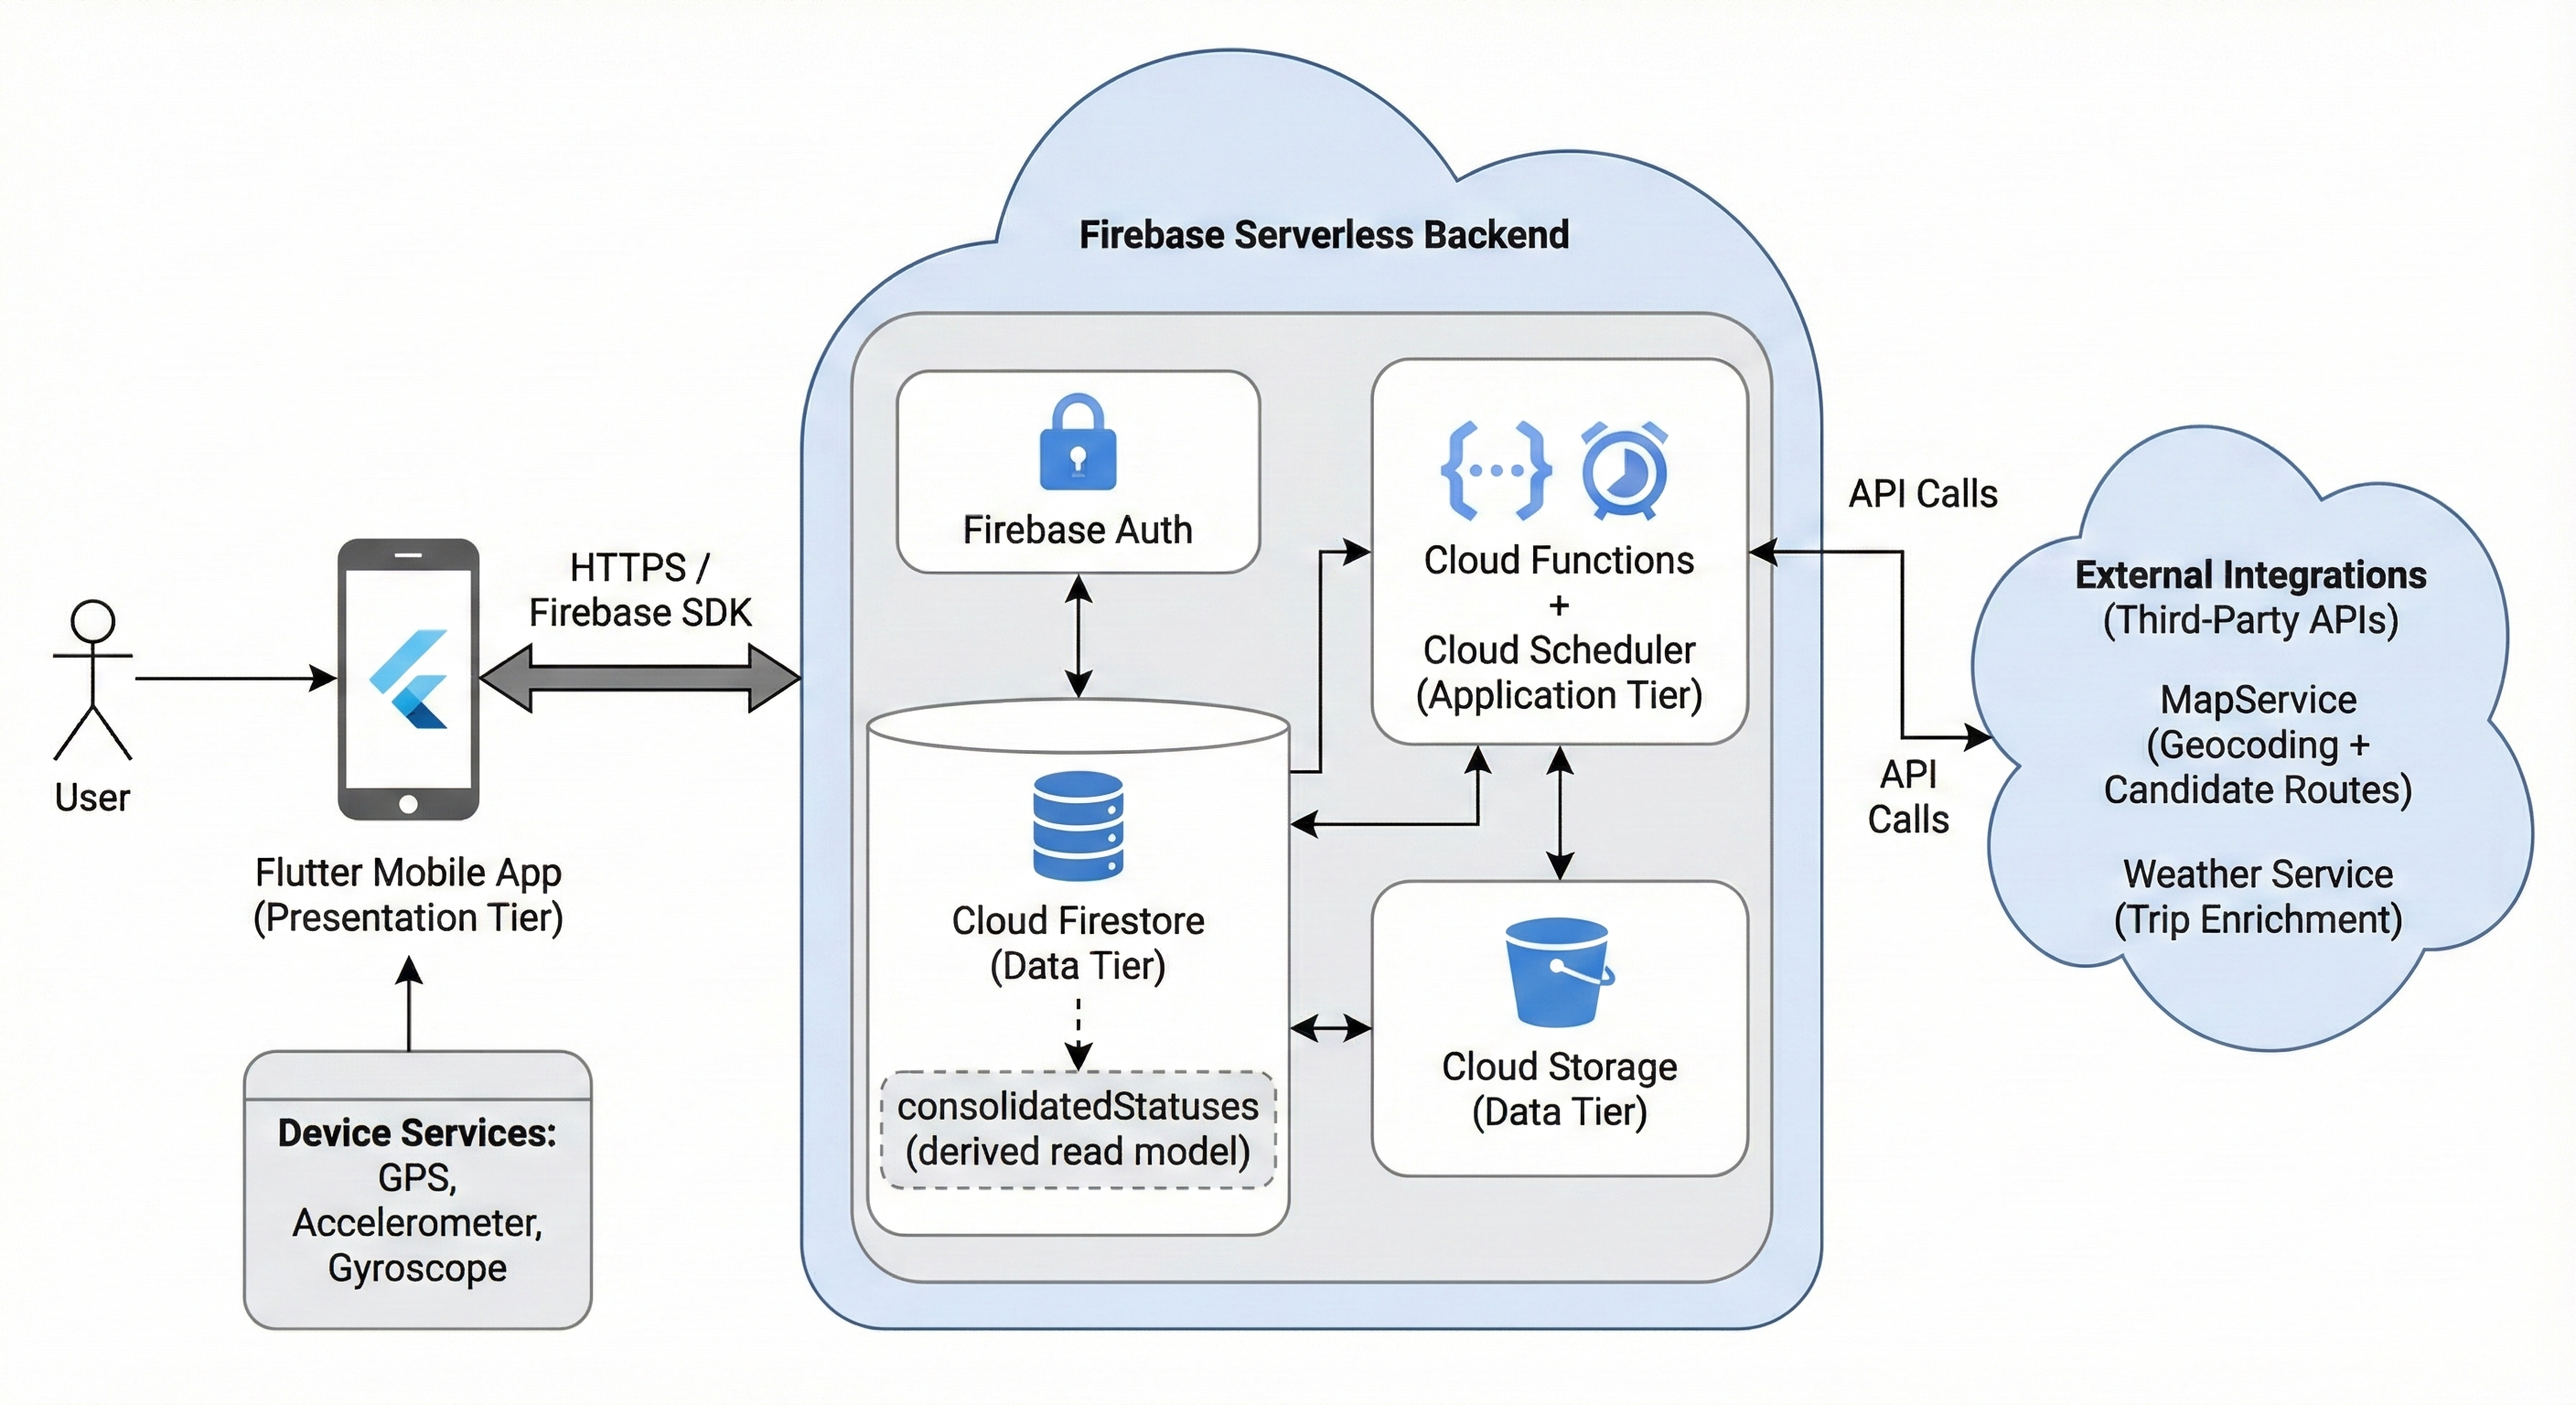
\includegraphics[width=\textwidth]{Images/Architectural overview.png}
\caption{\label{fig:architecutral_dig} Architectural Overview Diagram}
\end{figure}


\newpage

\subsection{Component View}
The system is organized into the following main components.

\begin{enumerate}
    \item \textbf{Flutter Mobile App (Presentation Tier)}: The Flutter client provides the user interface for registration and login, trip recording, contribution submission and route search. It interacts with Firebase services through the Firebase SDK over HTTPS. It also accesses device services such as GPS, accelerometer and gyroscope to collect trip traces and sensor signals that can support automatic detection workflows.

    \item \textbf{Firebase Authentication:}  Firebase Authentication manages user registration, login and session handling. It issues identity tokens that are used by clients to access protected backend resources according to Firestore Security Rules and Cloud Functions authorization checks.

        \begin{sidewaysfigure}
        \centering
        \includegraphics[width=\textwidth]{Images/component_view.jpg}
        \caption{\label{fig:domain_class_dig}Domain Class Diagram.}
        \end{sidewaysfigure}
    \item \textbf{Cloud Firestore (Data Tier):} Firestore stores the structured data required by BBP, including users, trips metadata, trip summaries, segment reports, obstacles, publishable flags and derived read models. Firestore is also used to support reactive UI updates where appropriate through real time listeners.
    \item \textbf{Cloud Storage (Data Tier):}  Cloud Storage stores larger objects, compressed location sequences and optional media attachments related to reports. Firestore stores references and metadata for these objects.
    \item \textbf{Cloud Functions and Cloud Scheduler (Application Tier):} Cloud Functions implement protected operations such as route scoring, report merging and generation of consolidated segment status. Functions also act as a controlled gateway to external services to prevent exposing API keys and to ensure consistent validation and rate limiting. Cloud Scheduler is used to trigger periodic maintenance and aggregation tasks such as recomputing consolidated statuses or cleaning up temporary records.
    \item \textbf{External Integrations (Third Party APIs):} BBP integrates with a map service for geocoding and route candidate generation between origin and destination. It also integrates with a weather service to enrich recorded trips with contextual conditions such as temperature, wind and precipitation.

\end{enumerate}


% \begin{figure}[H]
% \centering
% \includegraphics[width=\textwidth]{Images/component_view.jpg}
% \caption{\label{fig: component_dig} Component Diagram}
% \end{figure}






\newpage
\subsection{Deployment View}

BBP is deployed as a client serverless system.

\begin{enumerate}
    \item The Flutter application runs on end user mobile devices and communicates with Firebase over HTTPS using the Firebase SDK.

    \item The backend is deployed entirely on Firebase and Google Cloud managed infrastructure. Firestore and Cloud Storage store data, while Cloud Functions provide execution environments for application logic.
    \item External services are accessed by Cloud Functions, not directly by the mobile client, for operations that require secrets or controlled execution.

\end{enumerate}
This deployment minimizes backend administration, enables elastic scaling and supports a pay per use model.

\begin{figure}[H]
\centering
\includegraphics[width=0.35\textwidth]{Images/Deployment_view.png}
\caption{\label{fig:deployemnt_dig} Deployment Diagram} 
\end{figure}



\newpage
\subsection{Runtime View}
The runtime behavior of BBP can be described by considering how components collaborate to realize the core use cases.(UC1 to UC2)

\begin{enumerate}

    \item \textbf{User authentication and session establishment(UC1, UC2)}

        \begin{figure}[H]
        \centering
        \includegraphics[width=\textwidth]{Images/sequence_diagrams/UC1_page-0001.jpg}
        \caption{\label{fig:seqence_dig1} User Authentication Sequence Diagram}
        \end{figure}


        \begin{figure}[H]
        \centering
        \includegraphics[width=\textwidth]{Images/sequence_diagrams/UC2_page-0001.jpg}
        \caption{\label{fig:sequence_dig2} User Session Establishment Sequence Diagram}
        \end{figure}
    \begin{itemize}
        \item The user registers or logs in through the Flutter application.

        \item Firebase Authentication verifies credentials and returns an identity token.
        \item The client uses the token to access Firestore documents and callable or HTTPS Cloud Functions.
        

    \end{itemize}

    \item \textbf{Trip recording and storage(UC3)}
    \begin{itemize}
        \item The user starts trip recording in the Flutter application.
        \item The client reads GPS and sensor data at configured intervals.
        \item During recording, the client may compute lightweight statistics locally and stores intermediate data in memory.
        \item At the end of the trip, the client uploads trip metadata to Firestore and uploads the heavier trace payload to Cloud Storage.
        \item A Cloud Function may be triggered to compute additional derived statistics or to normalize trip structures for later visualization.
        
        \begin{figure}[H]
        \centering
        \includegraphics[width=0.65\textwidth]{Images/sequence_diagrams/UC3_page-0001.jpg}
        \caption{\label{fig:sequence_dig3} Trip Recording Sequence Diagram}
        \end{figure}


    \end{itemize}
    \item \textbf{Manual contribution workflow(UC4)}
    \begin{itemize}
        \item A registered user submits a path segment status or obstacle through the UI.
        \item The client writes the report into Firestore with a publishable flag selected by the user.
        \item A backend function validates the submission and may trigger aggregation updates for the affected segment.

        \begin{figure}[H]
        \centering
        \includegraphics[width=0.8\textwidth]{Images/sequence_diagrams/UC4_page-0001.jpg}
        \caption{\label{fig:sequence_dig4} Manual Contribution Workflow Sequence Diagram}
        \end{figure}
        
    \end{itemize}
    \item \textbf{Sensor assisted detection confirmation(UC5)}
    \begin{itemize}
        \item While recording, the client can detect candidate issues based on sensor signals and location context.
        \item Candidate issues are stored as private draft items for the user.
        \item The application prompts the user to confirm, correct or discard each candidate issue.
        \item Only confirmed and publishable items are written to the community visible collections.
        
        \begin{figure}[H]
        \centering
        \includegraphics[width=0.8\textwidth]{Images/sequence_diagrams/UC5_page-0001.jpg}
        \caption{\label{fig:sequence_dig5} Sensor Assisted Detection Confirmation Sequence Diagram}
        \end{figure}

    \end{itemize}
    \item \textbf{Route search, scoring and visualization(UC6)}
    \begin{itemize}
        \item The user specifies origin and destination in the Flutter application.
        \item The client requests candidate routes via a protected Cloud Function.
        \item The Cloud Function calls the external map service to obtain candidate routes and associated polyline or segment representations.
        \item The backend retrieves consolidated segment information from Firestore and computes a route score that combines quality and effectiveness factors.
        \item The ranked routes are returned to the client for visualization and selection.
        \item Generally, this behaviour reflects the formal cycling route research where candidate paths are ranked. Usually by a combined utility or attractiveness objective and sometimes under constraints. BBP implements a practical real time version of this idea for end users \cite{polimi_research_paper}.

        \begin{figure}[H]
        \centering
        \includegraphics[width=0.65\textwidth]{Images/sequence_diagrams/UC6_page-0001.jpg}
        \caption{\label{fig:sequence_dig6} Route Search and Scoring Sequence Diagram}
        \end{figure}

    \end{itemize}
    \item \textbf{Merging and consolidated status updates(UC7)}
    \begin{itemize}
        \item When multiple reports affect the same segment, a backend function computes a consolidated status by applying freshness and confirmation logic.
        \item The consolidated read model is stored in a dedicated collection for efficient querying during route scoring and map rendering.
        \item Periodic recomputation may be scheduled via Cloud Scheduler to ensure consistency and to incorporate aging policies.
    
        \begin{figure}[H]
        \centering
        \includegraphics[width=\textwidth]{Images/sequence_diagrams/UC7_page-0001.jpg}
        \caption{\label{fig:sequence_dig7} Merging and Consolidated Status Update Sequence Diagram}
        \end{figure}
    \end{itemize}

\end{enumerate}



\subsection{Interface View}
BBP exposes interfaces between the client and the backend through Firebase SDK operations and Cloud Functions endpoints.

\begin{enumerate}
    \item \textbf{Client to Firebase Authentication:} Registration, login, password reset and token management are handled through the Firebase SDK.
    \item \textbf{Client to Firestore:} The client reads and writes documents according to Security Rules. Typical reads include user profile, trip list, trip summaries and route results. Typical writes include trip metadata, user preferences and user owned contribution drafts.
    \item \textbf{Client to Cloud Functions:} Cloud Functions provide APIs for operations requiring server side enforcement or third party integrations such as:
        \begin{itemize}
            \item Requesting candidate routes and performing route scoring
            \item Triggering consolidation and merge processes
            \item Performing validation and normalization of submissions
            \item Retrieving weather enrichment for trips when needed
        \end{itemize}
    \item \textbf{Cloud Functions to External APIs:} Cloud Functions call map and weather services using secure stored credentials. Responses are transformed into BBP domain structures before being persisted or returned.
\end{enumerate}




\subsection{Architectural Style and Patterns}
BBP adopts the following architectural styles and patterns:
\begin{enumerate}
    \item \textbf{Serverless architecture:} The backend relies on managed services and function based computation. This supports scalability and reduces infrastructure management.
    \item \textbf{Layered architecture:} Presentation logic resides on the Flutter client, application logic resides in Cloud Functions and persistence is handled by Firestore and Cloud Storage.
    \item \textbf{Event driven and reactive data access:} Firestore enables real time updates for relevant UI elements. Backend functions may be triggered by database events to update derived models.
    \item \textbf{CQRS inspired read models:} Consolidated segment status is stored in a dedicated collection as a derived read model optimized for frequent route scoring queries. This reduces repeated computation during interactive route searches.
\end{enumerate}

\subsection{Data Management}

BBP stores and manages data in a way that supports both personal trip logs and community maintained path quality.
\begin{enumerate}
    \item \textbf{Core entities stored in Firestore}
    \begin{itemize}
        \item Users and preferences
        \item Trips metadata and summary statistics
        \item Segment reports and obstacle reports with publishable or private designation
        \item Consolidated segment statuses used for scoring and map visualization
    \end{itemize}
    \item \textbf{Large payloads stored in Cloud Storage}
    \begin{itemize}
        \item Full GPS traces and dense samples
        \item Optional attachments related to reports
    \end{itemize}
    \item \textbf{Derived read models:} Consolidated segment statuses are maintained in a separate collection to support low latency reads during route scoring. Updates occur when new publishable reports arrive and may also be recomputed periodically.
    \item \textbf{Consistency model:} Firestore provides strong consistency for document reads, while derived models may be eventually consistent depending on trigger timing. The design prioritizes user facing responsiveness, while ensuring that consolidation logic converges to stable results.
\end{enumerate}





\subsection{Security Design}

Security is enforced through a combination of authentication, authorization rules and controlled server side execution.

\begin{enumerate}
    \item \textbf{Authentication:} Users authenticate through Firebase Authentication. Identity tokens are required for operations tied to personal data or contributions.
    \item \textbf{Authorization:} Firestore Security Rules restrict reads and writes based on user identity and ownership. Private trip data and private candidate issues are accessible only to their owners. Community visible publishable data is readable according to the intended visibility rules.
    \item \textbf{Protected operations:} Cloud Functions encapsulate operations that require secrecy, controlled validations or merging logic. External API keys are not embedded in the client.
    \item \textbf{Privacy by design:} The system maintains a strict separation between private user data and publishable community data. Publication is always an explicit user choice.
\end{enumerate}



\subsection{Design Decisions and Rationale}
The chosen architecture reflects the project constraints and the expected usage patterns.


\begin{enumerate}
    \item Firebase services provide a consistent ecosystem for authentication, real time data access and secure server side logic, reducing integration complexity.
    \item Cloud Functions centralize business rules such as merging and scoring, which improves integrity and prevents client side manipulation.
    \item The use of a consolidated status read model improves performance during route searches by avoiding expensive aggregation at query time.
    \item Cloud Storage is used for large traces to keep Firestore efficient and to reduce document size constraints.
    \item External API calls are handled server side to protect secrets, manage quotas and provide a stable contract to the client.
\end{enumerate}


%------------------------------------------------------------------------------------------------------------------------------------------------
\clearpage
{\color{Blue}{\section{User Interface Design}}}
\label{sect:ui_desing}
\noindent 
This section maps UI screens to RASD use cases.\vspace{0.3cm} 
\subsection{Registration}
\begin{itemize}
  \item Registration form
  \item Login form
  \item Blocked account message
\end{itemize}

\begin{figure}[H]
\centering
\includegraphics[width=0.5\textwidth]{Images/figma_diagrams/Registration_page-0001.jpg}
\caption{\label{fig:figma_dig1} User Registration Screen}
\end{figure}

\newpage

\subsection{Dashboard}
\begin{itemize}
  \item Start recording
  \item Quick route search
  \item Recent trips
\end{itemize}

\begin{figure}[H]
\centering
\includegraphics[width=0.5\textwidth]{Images/figma_diagrams/Home_page-0001.jpg}
\caption{\label{fig:figma_dig2} Dashboard Screen}
\end{figure}

\newpage

\subsection{Trip Recording}
\begin{itemize}
  \item Start/Stop
  \item Stats (distance, duration, speed)
  \item Automatic mode indicator (if enabled)
\end{itemize}

\begin{figure}[H]
\centering
\includegraphics[width=0.5\textwidth]{Images/figma_diagrams/Trip Recording.png}
\caption{\label{fig:figma_dig3} Trip Recording Screen}
\end{figure}
\newpage

\subsection{Trip History \& Details}
\begin{itemize}
  \item List trips
  \item Details view: map, stats, weather snapshot
\end{itemize}

\begin{figure}[H]
\centering
\includegraphics[width=0.5\textwidth]{Images/figma_diagrams/Trip review_page-0001.jpg}
\caption{\label{fig:figma_dig4} Trip History and Details Screen}
\end{figure}

\newpage

\subsection{Manual Contribution}
\begin{itemize}
  \item Select/draw segment(s)
  \item Assign status
  \item Add obstacles
  \item Publishable/private toggle
  \item Edit/delete previous reports
\end{itemize}


\begin{figure}[H]
\centering
\includegraphics[width=0.5\textwidth]{Images/figma_diagrams/Contribute Paths (Manual).jpg}
\caption{\label{fig:figma_dig5} Manual Contribution Screen}
\end{figure}

\newpage

\subsection{Automatic Review}
\begin{itemize}
  \item Candidate list/map
  \item Confirm/reject/edit candidate
  \item Finalize
\end{itemize}

\begin{figure}[H]
\centering
\includegraphics[width=0.5\textwidth]{Images/figma_diagrams/automatic_detection_review.png}
\caption{\label{fig:figma_dig6} Automatic Detection Review Screen}
\end{figure}

\newpage

\subsection{Route Search \& Results}
\begin{itemize}
  \item Enter origin/destination
  \item Candidate list ordered by score
  \item Detail explanation
  \item Map overlay visualization (segment status + obstacles)
\end{itemize}

\begin{figure}[H]
\centering
\includegraphics[width=0.5\textwidth]{Images/figma_diagrams/Search path_page-0001.jpg}
\caption{\label{fig:figma_dig7} Route Search and Results Screen}
\end{figure}

\newpage

\subsection{Admin}
\begin{itemize}
  \item Block user
  \item Hide/remove report or obstacle
\end{itemize}

\begin{figure}[H]
\centering
\includegraphics[width=\textwidth]{Images/figma_diagrams/admin_screen_firebase.png}
\caption{\label{fig:figma_dig8} Admin Screen}
\end{figure}


%------------------------------------------------------------------------------------------------------------------------------------------------
\clearpage
{\color{Blue}{\section{Requirements Traceability}}}
\label{sect:requirements_traceability}
\subsection{Functional Requirements}
\paragraph{Trip Recording \& Statistics}
\begin{description}
    \item[\textbf{R1 - User registration}] 
    The system shall allow a user to create an account using an email (or federated login) and password.

    \item[\textbf{R2 - User login}] 
    The system shall allow a registered user to authenticate and access their personal data.

    \item[\textbf{R3 - Start trip recording}] 
    The system shall allow a logged-in user to start recording a new trip, initializing GPS logging and timing.

    \item[\textbf{R4 - Stop trip recording}] 
    The system shall allow the user to stop an ongoing trip and save it as a completed trip.

    \item[\textbf{R5 - Trip statistics}] 
    After a trip is saved, the system shall compute and store at least distance, duration and average speed.

    \item[\textbf{R6 - Trip history}] 
    The system shall allow a logged-in user to view the list of all recorded trips and open detailed views.

    \item[\textbf{R7 - Trip weather enrichment}] 
    For each trip, if the weather service is reachable, the system shall fetch and attach weather information based on time and location.
\end{description}

\paragraph{Manual Path Information}
\begin{description}
    \item[\textbf{R8 - Manual path creation}] 
    The system shall allow a logged-in user to select or draw a bike path using the map or by specifying street names.

    \item[\textbf{R9 - Segment status assignment}] 
    The system shall allow the user to set a status (optimal, medium, sufficient, requires maintenance, etc.) for each segment of a path.

    \item[\textbf{R10 - Obstacle creation}] 
    The system shall allow the user to create obstacles associated with a segment, specifying the obstacle type and a description.

    \item[\textbf{R11 - Publishability}] 
    The system shall allow the user to mark manual contributions as publishable or private.

    \item[\textbf{R12 - Edit manual contributions}] 
    The system shall allow users to edit or delete their previously submitted path reports.
\end{description}

\paragraph{Automatic path information}
\begin{description}
    \item[\textbf{R13 - Enable/disable automatic mode}] 
    The system shall allow a user to enable or disable automatic collection of sensor data for path quality detection.

    \item[\textbf{R14 - Sensor data logging}] 
    When automatic mode is enabled and a trip is being recorded, the system shall periodically sample accelerometer and gyroscope data and associate them with geographic positions.

    \item[\textbf{R15 - Detection of candidate obstacles}] 
    The system shall process sensor data and detect significant events (e.g., strong jolts) as candidate potholes or rough path segments.

    \item[\textbf{R16 - Candidate list presentation}] 
    After a trip ends, the system shall present the user with a list or map of candidate issues detected during that trip.

    \item[\textbf{R17 - User confirmation/correction}] 
    For each candidate, the user shall be able to confirm it, reject it, or edit its details (type, severity, or position) before it becomes a report.

    \item[\textbf{R18 - Conversion into reports}] 
    Confirmed candidates shall be stored as \textit{PathSegmentReport} objects associated with path segments. Rejected candidates shall not be stored as publishable data.
\end{description}

\paragraph{ Path search and visualization}
\begin{description}
    \item[\textbf{R19 - Public path search}] 
    The system shall allow any user, whether registered or not, to specify an origin and destination and request bike paths.

    \item[\textbf{R20 - Route computation}] 
    The system shall compute one or more route candidates using external map and routing services in combination with the internal path database.

    \item[\textbf{R21 - Path scoring}] 
    The system shall compute a score for each candidate path based on:
    \begin{itemize}
        \item Consolidated statuses of included segments.
        \item Severity and number of obstacles.
        \item Route effectiveness (e.g., distance, elevation, number of turns).
    \end{itemize} 
    \item[\textbf{R22 - Ordered path list}] 
    The system shall present candidate paths ordered by decreasing score.

    \item[\textbf{R23 - Path visualization}] 
    The system shall visualize a selected path on a map with overlays representing segment status and reported obstacles.
\end{description}

\paragraph{Data Merging}
\begin{description}
    \item[\textbf{R24 - Segment report storage}] 
    The system shall store all PathSegmentReports with timestamps and user identifiers.

    \item[\textbf{R25 - Periodic merging}] 
    The system shall periodically recompute the consolidated status of each segment based on all available reports.

    \item[\textbf{R26 - Freshness handling}] 
    The merging process shall weigh newer reports more heavily than older ones.

    \item[\textbf{R27 - Majority handling}] 
    If multiple reports with similar freshness disagree, the consolidated status shall follow the majority assessment (e.g., by count or weighted count).
\end{description}

\paragraph{Administration and data quality}
\begin{description}
    \item[\textbf{R28 - User Blocking}] 
    The system shall allow administrators to block users who repeatedly submit obviously false data.

    \item[\textbf{R29 - Data Removal}] 
    Administrators shall be able to remove or hide problematic reports.
\end{description}


\newpage

% Ragged-right p-columns (prevents most Underfull \hbox in tables)
\newcolumntype{P}[1]{>{\RaggedRight\arraybackslash}p{#1}}

% --- Your table (rectified) ---
\subsection{Requirements Traceability Table}

\renewcommand{\arraystretch}{1.15}
\setlength{\tabcolsep}{4pt}

% optional: helps TeX avoid both underfull/overfull in tight tables
\begingroup
\sloppy
\setlength{\emergencystretch}{1.5em}

\begin{longtable}{|P{1.1cm}|P{3.3cm}|P{2.2cm}|P{3.0cm}|P{5.1cm}|}
\caption{Requirements traceability table}
\label{tab:req-traceability}\\
\hline
\textbf{Req ID} & \textbf{Requirement (short)} & \textbf{Flutter Module(s)} & \textbf{Firebase Services} & \textbf{Main Data/Artifacts} \\
\hline
\endfirsthead

\hline
\textbf{Req ID} & \textbf{Requirement (short)} & \textbf{Flutter Module(s)} & \textbf{Firebase Services} & \textbf{Main Data/Artifacts} \\
\hline
\endhead



\endlastfoot

R1  & User registration & A1 & F1, F2 & \texttt{users/\{uid\}} \\
\hline
R2  & User login & A1 & F1, F2 & \texttt{users/\{uid\}} \\
\hline
R3  & Start trip recording & A2 & (F2 optional) & local GPS buffer \\
\hline
R4  & Stop trip recording & A2, A3 & F2, F3, (F4 optional) &
\texttt{trips/\allowbreak\{tripId\}} + trace file \\
\hline
R5  & Trip statistics & A2, A3 & F2, (F4 optional) & fields in \texttt{trips/\{tripId\}} \\
\hline
R6  & Trip history & A3 & F2 & query trips by uid \\
\hline
R7  & Trip weather enrichment & A3 & F4, F2 & \texttt{trips.weatherSnapshot} \\
\hline
R8  & Manual path creation & A4 & F2 & pathSegments, pathSegmentReports \\
\hline
R9  & Segment status assignment & A4 & F2 &
\seqsplit{pathSegmentReports.segmentStatus} \\
\hline
R10 & Obstacle creation & A4 & F2, (F3 optional) & obstacles (optional photo in Storage) \\
\hline
R11 & Publishability & A4 & F2 & publishable flag on reports and obstacles \\
\hline
R12 & Edit manual contributions & A4 & F2, (F4 validation optional) & update or delete own pathSegmentReports \\
\hline
R13 & Enable/disable automatic mode & A1, A2, A5 & F2 & \texttt{users.automaticModeEnabled} \\
\hline
R14 & Sensor data logging & A2 & (F2 optional), (F3 optional) & sensor samples + GPS tags \\
\hline
R15 & Detect candidate obstacles & A5 & (F4 optional) & candidate events (local or stored) \\
\hline
R16 & Candidate list presentation & A5 & none required & candidate UI list or map \\
\hline
R17 & User confirmation or correction & A5 & F2 & confirmed or edited candidate data \\
\hline
R18 & Conversion into reports & A5 & F2 & create pathSegmentReports and obstacles \\
\hline
R19 & Public path search & A6 & F2, F4 & read consolidated data + compute route \\
\hline
R20 & Route computation & A6 & F4 + external routing &
\seqsplit{computeRoutesAndScores()} + MapService \\
\hline
R21 & Path scoring & A6 & F4, F2 & uses consolidatedStatuses + obstacles \\
\hline
R22 & Ordered path list & A6 & F4 & sorted candidates returned \\
\hline
R23 & Path visualization & A6 & F2 & overlays from consolidated statuses + obstacles \\
\hline
R24 & Segment report storage & A4, A5 & F2 & pathSegmentReports with uid + timestamps \\
\hline
R25 & Periodic merging & none & F5, F4, F2 & refresh consolidatedStatuses \\
\hline
R26 & Freshness handling & none & F4, F2 & timestamp weighting in merge \\
\hline
R27 & Majority handling & none & F4, F2 & majority or weighted-majority merge rule \\
\hline
R28 & User blocking & A7 & F1 (role), F2, F4 & users.blocked + admin enforcement \\
\hline
R29 & Data removal or hide & A7 & F2, F4 & hide or delete report + recompute merge \\
\hline

\end{longtable}
\endgroup


\clearpage
{\color{Blue}{\section{Implementation, Integration and Test Plan
}}}
\label{sect:implementation_integration_test_plan}
\subsection{Overview and adopted strategies}
The implementation plan defines the order in which BBP is built, while the integration and test plan defines how BBP is assembled and validated step by step. The two plans must be consistent, because integration testing becomes effective only when it follows the same sequence used to combine components. BBP does not use a big bang integration approach, where all modules are integrated only at the end. Big bang provides late feedback and makes fault localization expensive.
Instead, BBP follows an incremental and iterative integration process where components are integrated and tested as soon as they are available.


The BBP adopts the following approach as our integration strategies:
\begin{enumerate}
    \item \textbf{Thread Based Integration:}  BBP integrates the system by delivering complete user visible features, each requiring cooperation among multiple modules. This provides early working functionality and reduces the need for artificial drivers compared to purely structural integration.
    \item \textbf{Bottom Up Integration inside each thread:} Within each feature, BBP integrates starting from the lower level elements such as data models, repositories, persistence and backend functions, then connects state management and UI. Bottom up integration reduces the need for stubs, but often requires drivers to exercise low level units, which BBP provides through repository and function level test harnesses.

    \item \textbf{Critical Modules First:} BBP prioritizes high risk modules early specifically GPS tracking, sensor sampling and candidate detection feasibility and MapService integration, so feasibility issues are discovered early.

\end{enumerate}

Testing in isolation often requires scaffolding because modules depend on other modules. BBP uses stubs and drivers when needed to simulate missing units during incremental integration.

\subsection{Implementation Plan}
BBP is divided into features to implement the thread based strategy. The RASD use cases and requirements are the critical components to implement. A feature is intended as a coherent functionality that becomes usable to the user and typically requires integration across several subcomponents.


Each feature has a significant outcome and provides a stable base for further development. The following are the identified features and the order of implementation feature-wise. 

\begin{enumerate}
    \item \textbf{F1 - Sign Up and Sign In (UC1, UC2, R1, R2):} Implementation of  registration and login through Auth, create user profiles in Firestore and enforce blocked user handling at login.
    \item \textbf{F2 - Trip Recording Core (UC3 partial, R3, R5 computation base):} Implementation of  the live trip tracking loop using GPS, including permission handling, start and stop controls, local buffering of GPS points and real time computation of core statistics while recording.
    \item \textbf{F3 - Trip Persistence, History and Details (UC3 completion and R4, R5, R6):} Persist completed trips to Firestore, upload traces to Cloud Storage and implement trip list and trip details views. This feature makes recorded trips durable and reviewable.
    \item \textbf{F4 - Weather Enrichment (UC3 extension, R7):}  Add optional weather enrichment after trip persistence is stable, storing weather snapshots in trip records when the service is reachable.
    \item \textbf{F5 - Manual Path Contributions (UC4, R8 to R12, R24 partially):} Implement map based segment selection or creation, segment status assignment, obstacle reporting, publishable or private selection and editing or deletion of own contributions.
    \item \textbf{F6 - Automatic Detection Review (UC5, R13 to R18):} Implement automatic mode settings, sensor sampling during trips, candidate detection, candidate review UI and conversion of confirmed candidates into reports and obstacles.
    \item \textbf{F7 - Route Search (UC6 part 1, R19, R20):} Implementation of origin and destination input, geocoding and retrieval of candidate routes from MapService. This feature focuses on obtaining feasible route candidates.
    \item \textbf{F8 - Path Scoring and Visualization (UC6 part 2, R21 to R23):} Implementation of segment mapping, retrieval of consolidated statuses and obstacles, scoring of candidates, ordered results list and map visualization with overlays.
    \item \textbf{F9 - Report Merging into Consolidated Status (UC7, R24 to R27):} Implement periodic merging with freshness weighting and majority resolution and maintain consolidatedStatuses as the derived read model used for fast scoring.
    \item \textbf{F10 - Administration and Moderation (R28, R29):} Implement admin operations to block users and hide or remove problematic reports and obstacles, enforced through roles, security rules and backend logic.
\end{enumerate}

\newpage
\subsection{Component Integration and Testing}

Integration testing focuses on the interaction between components and the correctness of their interfaces because many failures arise from inconsistent assumptions, misinterpreted parameters and unintended side effects across modules.

BBP integrates by feature threads and tests after each integration step rather than deferring testing to the end. It uses Firebase Emulator Suite for Auth, Firestore, Functions and  Storage to run repeatable integration tests, validate security rules and avoid dependence on a remote environment during continuous development. External services, MapService and Weather service are outside the system boundary. BBP therefore does not re-test their internal correctness, but it validates the integration points through stubs, controlled inputs and  failure mode testing such as timeouts.
\subsubsection{Integration steps by feature thread}
\begin{enumerate}
    \item \textbf{F1 - Sign Up and Sign In:}

        \begin{itemize}
            \item \textbf{Integrated components:} Auth UI, Firebase Authentication, Firestore user profiles, security rules for profile data.
            \item \textbf{Integration tests:} register, login, profile creation, blocked user access denial.

        \end{itemize}

        \begin{figure}[H]
        \centering
        \includegraphics[width=\textwidth]{Images/testing_images/F1_signup_signin_testing.png}
        \caption{\label{fig:testing_f1} Integration testing diagram for Feature Thread F1 (Sign Up \& Sign In) }
        \end{figure}
\newpage
        \item \textbf{F2 - Trip Recording Core:}
        \begin{itemize}
            \item \textbf{Integrated components:} GPS permission flow, GPS streaming, local buffer, real time statistics computation.

            \item \textbf{Integration tests:} start trip, confirm GPS points are received, confirm stats update, stop trip produces a completed in memory trip object even before persistence.
            \item \textbf{Drivers:} Simulated GPS streams for deterministic tests, plus at least one real device test for feasibility.

            \begin{figure}[H]
            \centering
            \includegraphics[width=\textwidth]{Images/testing_images/F2_trip_recording_core_testing.png}
            \caption{\label{fig:testing_f2} Integration testing diagram for Feature Thread F2 (Trip Recording Core) }
            \end{figure}

        \end{itemize}
        \newpage
        \item \textbf{F3 - Trip Persistence, History and Details:}
            \begin{itemize}
                \item \textbf{Integrated components:} Firestore trip writes, Storage trace upload, trip list query by uid, trip details rendering.

                \item \textbf{Integration tests:} Stopping a trip creates trips/{tripId} and uploads a trace, trip history displays correct items, opening a trip shows stored stats and trace link.

            \begin{figure}[H]
            \centering
            \includegraphics[width=\textwidth]{Images/testing_images/F3_trip_persistence_history_testing.png}
            \caption{\label{fig:testing_f3} Integration testing diagram for Feature Thread F3 (Trip Persistence, History and Details) } 
            \end{figure}            
        \end{itemize}

        \newpage

        \item \textbf{F4 - Weather Enrichment:}
            \begin{itemize}
                \item \textbf{Integrated components:} weather client wrapper and trip update pipeline.

                \item \textbf{Integration tests:} reachable weather provider stores snapshot, unreachable provider results in trip stored without weather, with a clear fallback state.

            \begin{figure}[H]
            \centering
            \includegraphics[width=\textwidth]{Images/testing_images/F4_weather_enrichment_testing.png}
            \caption{\label{fig:testing_f4} Integration testing diagram for Feature Thread F4 (Weather Enrichment) } 
            \end{figure}            

            \end{itemize}
            \newpage
        \item \textbf{F5 - Manual Path Contributions:}
            \begin{itemize}
                \item \textbf{Integrated components:} segment creation or selection, report creation, obstacle creation, publishable or private logic, edit and delete own reports.

                \item \textbf{Integration tests:} create publishable reports and verify guest visibility rules, create private reports and verify only owner access, edit and delete restrictions validated by rules tests.

            \begin{figure}[H]
            \centering
            \includegraphics[width=\textwidth]{Images/testing_images/F5_manual_path_contributions_testing.png}
            \caption{\label{fig:testing_f5} Integration testing diagram for Feature Thread F5 (Manual Path Contributions) } 
            \end{figure}            

            \end{itemize}

            \newpage

        \item \textbf{F6 - Automatic Detection Review:}
            \begin{itemize}
                \item \textbf{Integrated components:} ensor sampling with GPS tagging, candidate detector, candidate review UI, conversion into reports and obstacles.


                \item \textbf{Integration tests:} candidate list produced deterministically using prerecorded sensor traces, confirm creates stored artifacts, reject creates none, edits modify stored artifacts.


            \begin{figure}[H]
            \centering
            \includegraphics[width=\textwidth]{Images/testing_images/F6_auto_detection_review_testing.png}
            \caption{\label{fig:testing_f6} Integration testing diagram for Feature Thread F6 (Automatic Detection Review) } 
            \end{figure}            

            \end{itemize}
            \newpage
        \item \textbf{F7 - Route Search:}
            \begin{itemize}
                \item \textbf{Integrated components:}origin and destination UI, geocoding, candidate route retrieval from MapService.

                \item \textbf{Integration tests:} valid locations return candidates, invalid address fails gracefully, timeouts handled with fallback messages.

                \item \textbf{Stubs:} MapService stub used for deterministic automated tests, replaced by real MapService for system tests.


            \begin{figure}[H]
            \centering
            \includegraphics[width=\textwidth]{Images/testing_images/F7_route_search_testing.png}
            \caption{\label{fig:testing_F7} Integration testing diagram for Feature Thread F7 (Route Search) }
            \end{figure}            

            \end{itemize}
            \newpage
            
        \item \textbf{F8 - Path Scoring and Visualization:}
            \begin{itemize}
                \item \textbf{Integrated components:}segment mapping, retrieval of consolidatedStatuses and obstacles, scoring logic, sorted list, map overlays.

                \item \textbf{Integration tests:} seeded Firestore dataset produces predictable scores, verify ordering by score, verify overlays match consolidated statuses and obstacles, verify guest sees only publishable and non hidden data.

            \begin{figure}[H]
            \centering
            \includegraphics[width=\textwidth]{Images/testing_images/F8_scoring_visualization_testing.png}
            \caption{\label{fig:testing_F8} Integration testing diagram for Feature Thread F8 (Path Scoring and Visualization) } 
            \end{figure}           

            \end{itemize}

            \newpage

        \item \textbf{F9 - Report Merging into Consolidated Status:}
            \begin{itemize}
                \item \textbf{Integrated components:} scheduled merge function, freshness weighting, majority resolution, consolidatedStatuses updates.

                \item \textbf{Integration tests:} seed reports with known timestamps and statuses, execute merge manually in emulator, verify consolidated result, verify hidden and private items excluded.


            \begin{figure}[H]
            \centering
            \includegraphics[width=\textwidth]{Images/testing_images/F9_report_merging_testing.png}
            \caption{\label{fig:testing_F9} Integration testing diagram for Feature Thread F9 (Report Merging into Consolidated Status) } 
            \end{figure}           

            \end{itemize}

            \newpage

        \item \textbf{F10 - Administration and Moderation:}
            \begin{itemize}
                \item \textbf{Integrated components:}  admin restricted UI, admin Cloud Functions, rule enforcement, optional audit logging.


                \item \textbf{Integration tests:} only admin can block users, blocked users cannot contribute, admin hide and remove excludes data from consolidated results after merge.

            \begin{figure}[H]
            \centering
            \includegraphics[width=\textwidth]{Images/testing_images/F10_admin_moderation_testing.png}
            \caption{\label{fig:testing_F10} Integration testing diagram for Feature Thread F10 (Administration and Moderation) } 
            \end{figure}           

            \end{itemize}
\end{enumerate}
\subsection{System Testing}
System testing validates BBP as a whole, using the RASD use cases as scenarios. The test environment is kept as close as possible to production, especially for GPS, sensors and  external services.

System tests are executed after each major feature thread becomes stable and  repeated as regression tests as the system grows.
\subsubsection{Functional System tests by use case}
\begin{enumerate}
    \item \textbf{UC1 - Registration}
        \begin{itemize}
            \item Valid registration creates Auth user and Firestore profile
            \item Invalid email or password rejected
            \item Duplicate email rejected
        \end{itemize}
        \newpage
    \item \textbf{UC2 - Login}
        \begin{itemize}
            \item Correct credentials allow access
            \item Wrong credentials rejected
            \item Blocked user denied after profile check
        \end{itemize}
    \item \textbf{UC3 - Record Trip}
        \begin{itemize}
            \item Permission denied prevents recording
            \item GPS unavailable handled safely
            \item Normal trip produces saved trip and trace when persistence is enabled
            \item Trip history shows new trip and details
            \item Weather reachable adds weather snapshot, weather unreachable still stores trip
        \end{itemize}
    \item \textbf{UC4 - Manual Path Contribution}
        \begin{itemize}
            \item Create segment reports for each status
            \item Add obstacles and verify correct storage and visualization
            \item Publishable contributions visible to guests, private contributions visible only to owner
            \item Edit and delete own contributions, not others’ contributions
        \end{itemize}
    \item \textbf{UC5 - Automatic Detection Review}
        \begin{itemize}
            \item Candidate detection produces list
            \item Confirm creates PathSegmentReport and obstacle when applicable
            \item Reject creates nothing
            \item Edit modifies stored data before publishing
        \end{itemize}
    \item \textbf{UC6 - Search Route}   
        \begin{itemize}
            \item Route search returns candidate routes for valid origin and destination
            \item Invalid address fails geocoding
            \item MapService timeout handled gracefully
            \item Scoring returns ordered list by decreasing score
            \item Selected route shows overlays matching consolidated statuses and obstacles
        \end{itemize}
    \item \textbf{UC7 - Merge}
        \begin{itemize}
            \item Merge updates consolidatedStatuses after new reports
            \item Freshness weighting influences result
            \item Majority rule followed
            \item Hidden and private reports excluded
        \end{itemize}

\end{enumerate}

\subsubsection{Non Functional System testing types}
BBP includes performance, load and stress testing at system level.
\begin{enumerate}
    \item Performance testing targets route scoring latency and overlay loading times.
    \item Load testing targets repeated route searches and repeated reads of consolidated status data.
    \item Stress testing targets failure and degraded conditions such as network loss or external service failure, ensuring BBP degrades gracefully and recovers.
\end{enumerate}

\subsection{Security tests and regression policy}
Security and access control testing is treated as continuous integration work rather than a one time activity:
\begin{enumerate}
    \item Guests cannot write any Firestore data
    \item Users can only modify their own trips and contributions
    \item Only admins can block users and hide or remove content
    \item Blocked users cannot submit publishable contributions
\end{enumerate}

Every defect found during integration or system testing is converted into a regression test, so the same fault does not reappear in the further tests. This supports incremental development and keeps integration stable as new features are added.


%------------------------------------------------------------------------------------------------------------------------------------------------
\clearpage
{\color{Blue}{\section{Effort Spent}}}
\label{sect:effort}
\begin{table}[H]
\centering
\begin{tabular}{|l|c|c|c|c|}
\hline
\textbf{Team Member} & 
\makecell{\textbf{Jayasurya}\\ \textbf{Marasani}} & 
\makecell{\textbf{Arunkumar}\\ \textbf{Murugesan}} & 
\makecell{\textbf{Sneharajalakshmi}\\ \textbf{Palanisamy}} & 
\makecell{\textbf{Section}\\ \textbf{Total}} \\
\hline
\textbf{Introduction}          & 3  & 3 & 3 & 9 \\
\hline
\textbf{Architecture}         & 10  & 10 & 10  & 30\\
\hline
\textbf{UI Design} & 7  & 7 & 8  & 22\\
\hline
\textbf{Requirements Traceability} & 8 & 8 & 8  & 24\\
\hline
\makecell[l]{\textbf{Implementation, } \\ \textbf{Integration and Test Plan}} & 13 & 12 & 11  & 36\\
\hline
\textbf{Total} & \textbf{41} & \textbf{40} & \textbf{40} & \textbf{121}\\
\hline
\end{tabular}
\caption{\label{tab:effort_balanced}Effort spent per member }
\end{table}



The table as shown in Table.~\ref{tab:effort_balanced}  displays the number of hours each group member spent on the various sections of the document. Please note that the division is only approximate and each section still required the colloboration of all team members.


%------------------------------------------------------------------------------------------------------------------------------------------------
\clearpage
\addcontentsline{toc}{section}{References}
% \bibliographystyle{plain}

% \bibliography{main}

\begin{thebibliography}{99}
\bibitem{valenzuela2023bicycle}
Valenzuela, A., Lopes, A., Rescarolli, M., Pazin, J., and Rech, C.
\newblock Analysis of the quality of bicycle paths and their relationship with bicycle use in Florianópolis.
\newblock \emph{Journal of Physical Education}, vol.~34, article~13, 2023.
\newblock doi:10.4025/jphyseduc.v34i1.3428.

\bibitem{polimi_research_paper}
Černá, A., Černý, J., Malucelli, F., Nonato, M., Polena, L., and Giovannini, A.
\newblock Designing optimal routes for cycle-tourists.
\newblock \emph{Transportation Research Procedia}, vol.~3, pp.~856--865, 2014.
\newblock doi:10.1016/j.trpro.2014.10.064.


\bibitem{figma}
Figma, Inc.
\newblock \textit{Figma: Collaborative Interface Design Tool}.
\newblock \url{https://www.figma.com}.


\bibitem{chatgpt}
OpenAI.
\newblock \textit{ChatGPT (used for paraphrasing)}.
\newblock \url{https://chatgpt.com}.

\bibitem{planttext}
PlantText.
\newblock \textit{PlantText: Online Text Editor for Writing and Notes}.
\newblock \url{https://www.planttext.com}.

\bibitem{overleaf}
Overleaf.
\newblock \textit{Overleaf: Online \LaTeX\ Editor}.
\newblock \url{https://www.overleaf.com/}.


\end{thebibliography}

%------------------------------------------------------------------------------------------------------------------------------------------------




\end{document}
